%%%%%%%%%%%%%%%%%%%%%%%%%%%%%%%%%%%%%%%%%
% Beamer Presentation
% LaTeX Template
% Version 1.0 (10/11/12)
%
% This template has been downloaded from:
% http://www.LaTeXTemplates.com
%
% License:
% CC BY-NC-SA 3.0 (http://creativecommons.org/licenses/by-nc-sa/3.0/)
%
%%%%%%%%%%%%%%%%%%%%%%%%%%%%%%%%%%%%%%%%%

%----------------------------------------------------------------------------------------
%	PACKAGES AND THEMES
%----------------------------------------------------------------------------------------

\documentclass[aspectratio=169]{beamer}
\usepackage[utf8]{inputenc}
\usepackage{booktabs}
\usepackage{graphicx}
\usepackage{array}
\usepackage{caption}
\usepackage{threeparttable}
\usepackage{lscape}
\usepackage{import}
\usepackage{multirow, array}
\usepackage{amsmath}
\usepackage{csvsimple}
\usepackage{siunitx}
\usepackage{subfigure}
\usepackage{filecontents}
\newenvironment{wideitemize}{\itemize\addtolength{\itemsep}{10pt}}{\enditemize}
\usepackage{appendixnumberbeamer}
\usepackage{float}
\usepackage{amsmath}  
\usepackage{tikz,pgfplots}
\usepackage{tkz-fct}
\usepackage{amsthm}
\pgfplotsset{compat=1.10}
\usepgfplotslibrary{fillbetween}
\newcommand{\vertLineFromPoint}[1]{
  \draw[dashed] 
  (#1) -- (#1|-{rel axis cs:0,0})
}
\newcommand{\horLineFromPoint}[1]{
  \draw[dashed] 
  (#1) -- (#1-|{rel axis cs:0,0})
}
\mode<presentation> {
\AtBeginSection[]
{
    \begin{frame}
        \frametitle{Table of Contents}
        \tableofcontents[currentsection]
    \end{frame}
}

% The Beamer class comes with a number of default slide themes
% which change the colors and layouts of slides. Below this is a list
% of all the themes, uncomment each in turn to see what they look like.

%\usetheme{default}
%\usetheme{AnnArbor}
%\usetheme{Antibes} -
%\usetheme{Bergen}
%\usetheme{Berkeley}
%\usetheme{Berlin}
\usetheme{Boadilla}
%\usetheme{CambridgeUS}
%\usetheme{Copenhagen} -
%\usetheme{Darmstadt}
%\usetheme{Dresden}
%\usetheme{Frankfurt}
%\usetheme{Goettingen}
%\usetheme{Hannover}
%\usetheme{Ilmenau}
%\usetheme{JuanLesPins}
%\usetheme{Luebeck}
%\usetheme{Madrid}
%\usetheme{Malmoe}
%\usetheme{Marburg}
%\usetheme{Montpellier}
%\usetheme{PaloAlto}
%\usetheme{Pittsburgh}
%\usetheme{Rochester} -
%\usetheme{Singapore}
%\usetheme{Szeged}
%\usetheme{Warsaw}

% As well as themes, the Beamer class has a number of color themes
% for any slide theme. Uncomment each of these in turn to see how it
% changes the colors of your current slide theme.

%\usecolortheme{albatross}
%\usecolortheme{beaver}
%\usecolortheme{beetle}
%\usecolortheme{crane}
%\usecolortheme{dolphin}
%\usecolortheme{dove}
%\usecolortheme{fly}
%\usecolortheme{lily}
%\usecolortheme{orchid}
%\usecolortheme{rose}
%\usecolortheme{seagull}
%\usecolortheme{seahorse}
%\usecolortheme{whale}
%\usecolortheme{wolverine}

%\setbeamertemplate{footline} % To remove the footer line in all slides uncomment this line
\setbeamertemplate{footline}[frame number] % To replace the footer line in all slides with a simple slide count uncomment this line
\setbeamertemplate{theorems}[numbered]
\setbeamertemplate{navigation symbols}{} % To remove the navigation symbols from the bottom of all slides uncomment this line
}
\setbeamertemplate{caption}{\raggedright\insertcaption\par}
  \setbeamertemplate{enumerate items}[default]
\usepackage{graphicx} % Allows including images
\usepackage{booktabs} % Allows the use of \toprule, \midrule and \bottomrule in tables
%\usepackage {tikz}
\newtheorem*{theorem*}{Theorem}
\newtheorem*{lemma*}{Lemma}
\newtheorem*{proposition}{Proposition}
\newtheorem*{corollary*}{Corollary}
\newtheorem*{definition*}{Definition}
\DeclareMathOperator*{\argmin}{arg\,min}
\newtheorem*{assumption}{Assumption}
\usetikzlibrary {positioning}
% macro for inputting terminal nodes
\newcommand\term[2]{\node[below]at(#1){$#2$};}
%
%\usepackage {xcolor}

%----------------------------------------------------------------------------------------
%	TITLE PAGE
%----------------------------------------------------------------------------------------

\title[Incomplete]{Lecture 8: Incomplete Information} % The short title appears at the bottom of every slide, the full title is only on the title page

\author{Jacob Kohlhepp} % Your name
\institute[UCLA] % Your institution as it will appear on the bottom of every slide, may be shorthand to save space
{
Econ 101 \\ % Your institution for the title page
\medskip
}
\date{\today} % Date, can be changed to a custom date

\begin{document}

\begin{frame}
\titlepage % Print the title page as the first slide
\end{frame}

\begin{frame}{Introduction}
\begin{wideitemize}
    \item We will now relax the assumption of ``perfect information."
    \item We will allow economic actors to not know everything about a game.
    \item Example: A firm may not know the productivity/skill of a worker they hired.
    \item Example: A seller may not know how much a buyer values an item.
    \item Notice that we implicitly assumed complete information in Econ 11.

\end{wideitemize}
\end{frame}

\begin{frame}{A New Tool: Player Types}

\begin{wideitemize}
    \item One useful way to think about incomplete information is \textbf{player types.}
    \begin{definition}
    A player's \textbf{type} (t) describes all of the actions and information available to a player.
    \end{definition}
    \item A player knows their own type, but may be uncertain (or have beliefs about) other player's types.
    \item This fits well with labor market examples: we can think of models with a high skill and low skill type of worker, where high skill workers may have different outputs but also different payoffs then low skill.
    \item This also covers things like poker.
    \begin{enumerate}
        \item Set the type space (the set of possible types) to be all possible two card hands.
        \item Then which cards you have determines what payoffs you got from the flop, turn and river.
        \item Which cards you have also determine your belief about other player's cards.
        \item Your cards are your private information because only you know them for certain.
    \end{enumerate}
\end{wideitemize}
    
\end{frame}

\begin{frame}{A Simple Example: Wall Street vs Reddit}
    Consider the following game inspired by the GameStop situation.
    \begin{wideitemize}
        \item There are two players: a Wall Street trader (W) and an anonymous Reddit trader (R).
        \item W can either short or leave while R can either buy or not.
        \item Now for some incomplete information: R is either rational (with prob. p) or a rage trader (with prob. 1-p).
        \item Payoffs are as follows:
    \end{wideitemize}
    
     \begin{table}
    \begin{tabular}{c c}
     $t_r=$ rational & $t_r=$ rage\\
    \begin{tabular}{cc|c|c|}
      & \multicolumn{1}{c}{} & \multicolumn{2}{c}{ $R$}\\
      & \multicolumn{1}{c}{} & \multicolumn{1}{c}{$B$}  & \multicolumn{1}{c}{$N$} \\\cline{3-4}
      \multirow{2}*{ $W$}  & $S$ & $(-10,-1)$ & $(1,0)$ \\\cline{3-4}
      & $L$ & $(0,0)$ & $(0,1)$ \\\cline{3-4}
    \end{tabular} &
   \begin{tabular}{cc|c|c|}
      & \multicolumn{1}{c}{} & \multicolumn{2}{c}{ $R$}\\
      & \multicolumn{1}{c}{} & \multicolumn{1}{c}{$B$}  & \multicolumn{1}{c}{$N$} \\\cline{3-4}
      \multirow{2}*{ $W$}  & $S$ & $(-10,10)$ & $(1,0)$ \\\cline{3-4}
      & $L$ & $(0,1)$ & $(0,0)$ \\\cline{3-4}
    \end{tabular}
   
      \end{tabular}
  \end{table}
\end{frame}

\begin{frame}{A New Solution Concept}
\begin{wideitemize}
    \item Notice that we have introduced types, so there is another element involved in the game.
    \item Wall Street trader will trade differently depending on if he faces a rage Redditor or a rational Redditor.
    \begin{definition}
    A \textbf{Bayesian Nash Equilibrium} (BNE) is a strategy profile $\{s^*_1(t_1), s_2^*(t_2),...s_n^*(t_n)\}$ such that each strategy for each type of each player is a best response given beliefs about the other's player's types ($Pr(t_{-i}=t)$):
    \[\sum_{j} Pr(t_{-i}=t_j)U_i(s^*_i(t_i), s^*_{-i}(t_j)) \geq  \sum_{j} Pr(t_{-i}=t_j)U_i(s'_i(t_i), s^*_{-i}(t_j))\]
    for all types, all players, and all strategies $s_i'$.
    \end{definition}
    \item Lots of math. Bottomline: every player plays a best response given their type assuming all other players play a best response knowing their type.
\end{wideitemize}
\end{frame}

\begin{frame}{A New Solution Concept}
\begin{wideitemize}
    \item The definition can feel overwhelming, so just focus on the intuition.
    \item Bottomline: every player plays a best response given their type assuming all other players play a best response knowing their type.
    \item We must specify what different player types know about other player types.
    \item For example, does the Wall Street trader know what type of Redditor they face?
    \item Or is it uncertain? Generally we will assume that people know their own type and are ucnertain about other people's type.
    \item Uncertainty amounts to believing the person was randomly drawn from the population, or that "nature moves prior to the game."
    \item In our example, the Wall Street trader believes the Redditor is rational with probability $p$.
    
\end{wideitemize}
\end{frame}

\begin{frame}{Applying BNE to GameStop}

See handwritten notes.\pause
\begin{wideitemize}
    \item In terms of technique this really just involved a few more steps.
    \item In terms of interpretation: Wall Street plays against an average of the two types.
    \item We can ask: would the rational Redditor prefer if Wall Street new their type?
    \item Would the rage Redditor prefer if Wall Street new their type?
    \item I highly recommend reviewing the tragedy of the commons example in N\&S (Example 8.6)
\end{wideitemize}
    
\end{frame}

\begin{frame}{Sequential Games with Incomplete Information}
\begin{wideitemize}
    \item The idea of types and incomplete information becomes more interesting and powerful when we add sequential moves.
    \item Why? Because then the actions of other players tell us something about their types.
    \item This is idea is called \textbf{signaling}, because observable actions serve as a signal of private information.
    \item Example: Going to college tells an employer you have some level of analytical ability/intelligence (this is the main example we will look at).
\end{wideitemize}
    
\end{frame}



\begin{frame}{Another Tool: Bayes' Rule}

\begin{wideitemize}
    \item In order to understand how a belief should be updated based on new information (education choice) we need Bayes' Rule.
    
    \begin{theorem}
    Given two events A and B Bayes' Rule states that:
    \[Pr(A | B) = \frac{Pr(A \& B)}{Pr(B)} = \frac{Pr(B | A)Pr(A)}{Pr(B)} \]
    \end{theorem}
    \item $Pr(A|B)$ reads the probability of A given B.
    \item Generally $A$ is the type of other player, and $B$ is some action taken by other player.
    \item In equilibrium, sometimes different types play different strategies which makes the actions a signal.
\end{wideitemize}
    
\end{frame}
\begin{frame}{Final Equilibrium Concept: Perfect Bayesian Equilibrium}
    \begin{wideitemize}
        \item Like when we added sequential moves with Nash Equilibrium, we need to refine BNE.
        \item Specifically we must say how beliefs change in response to actions.
        
        \begin{definition}
        A strategy profile $\{s_1^*(t_1), ...,s_n^*(t_n)\}$ and beliefs are a \textbf{Perfect Bayesian Nash Equilibrium} if:
        \begin{enumerate}
            \item at each information set players strategies maximize utility given beliefs.
            \item at each information set beliefs are determined by Bayes' rule where possible (given equilibrium strategies).
        \end{enumerate}
        \end{definition}
    \end{wideitemize}
\end{frame}


\begin{frame}{The Monty Hall Problem (Simple Deal or No Deal)}
    \begin{columns}[T] % align columns
\begin{column}{.63\textwidth}
\begin{wideitemize}
    \item A game show host gives you the option of picking one of three doors.
    \item One has a car, two have goats. Assume 1/3 prob. of car behind each door. Assume host knows which door has the car. Assume host can't open your door and randomizes when two other doors both have goats.
    \item You pick door 2. Host opens one of the unopened doors and reveals a goat.
    \item You can now either switch to the unopened door or stay. Which do you choose? (answer in survey)
\end{wideitemize}
\end{column}%
\hfill%
\begin{column}{.44\textwidth}
\resizebox{\textwidth}{!}{
  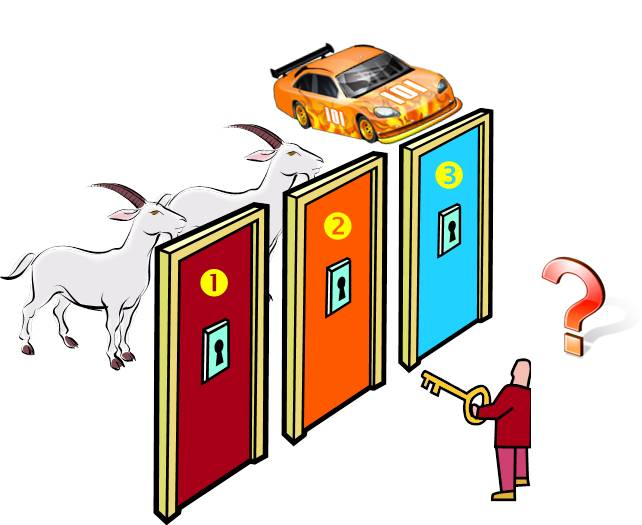
\includegraphics{monty-hall.jpg}
  
}
\end{column}%
\end{columns}

  \hfill Source: DesiSpeaks
\end{frame}

\begin{frame}{Solving Monty Hall}{Host Knows Nothing}

Assume first that the host does not know the location of the car. Which door should you choose to maximize your probability of finding the car? (fill in)

\vspace{5.5cm}

\vspace{6cm}

    
\end{frame}


\begin{frame}{Solving Monty Hall}{Host is Informed, Host Avoids Embarrassment}

We say the host is embarrassed if she opens a door with a car behind it. We say the host is embarrassed if she opens a door with a car behind it.Which door should you choose? (fill in)

\vspace{5.5cm}

    
\end{frame}

\begin{frame}{Solving Monty Hall}{Host is Informed, Host Is a Class Clown}

 Suppose now that the host does not care about being embarrassed. She is indifferent between revealing a goat or a car. Which door should you choose? (fill in)

\vspace{5.5cm}

    
\end{frame}

\begin{frame}{Insights from Monty Hall}

\begin{wideitemize}
    \item The first solution is the one most people give when asked. It ignores the fact that the host is privately informed.\footnote{We can show that as long as the host knows just a little bit more than the contestant, this answer is wrong.}
    
    \item The second is the solution given by Vos Savant and is seen as the correct answer.
    
    \item The third solution, which is similar to the first, is still considered wrong because the assumption is unreasonable. But it illustrates a subtle point.
    
    \begin{wideitemize}
        \item The second solution requires an assumption about the host's behavior.
        \item It is not enough that the host has private information.
        
        \item For the door opening to be informative about the car, there must be a \textbf{signaling cost.}
        \item In the Monty Hall problem, this is embarrassment or obligation or something on the host's end.
    \end{wideitemize}
\end{wideitemize}
    
\end{frame}


\begin{frame}{Spence Job Market Signaling}

\begin{wideitemize}
    \item We now consider a model developed by Spence, for which he won the Nobel Prize.
    \item Two players: a firm and a worker.
    \item Worker is either high-skill ($t=H$) with prob. $p$ or low-skill ($t=L$) with prob. $1-p$.
    \item The firm cannot observe worker type.
    \item Profit from hiring low-skill is 0 and high-skill is $\pi>0$
    \item At $t=1$ the worker can acquire education at cost $c_H$ if high type and $c_L$ if low-type.
    \item At $t=2$ after observing education the firm either hires or not at the wage $w$.\footnote{For simplicity we assume $\pi -w>0$ and that wage is not chosen by the firm.}
    \item Assume: the cost of education satisfies: $c_L>w>c_H$.
\end{wideitemize}
    
\end{frame}

\begin{frame}{Spence Job-market Signaling}

\begin{wideitemize}
    \item We now draw the game tree. See handwritten notes.
    \item In the drawing, note the information sets.
\end{wideitemize}
    
\end{frame}


\begin{frame}{Interpreting Job-market Signaling}

\begin{wideitemize}
    \item The game highlights how education can be useful even if it imparts no useful skills.
    \item Note that the separating equilibrium is inefficient: education is wasteful, and we could make everyone better off if we could costlessly signal type.
    \item The results of the model extend to cases where education also imparts skill.
    \item This model was crucial in separating the human capital vs the signaling value of education.
    \item  This led to the realization that we need to be careful when we estimate the returns to education.
    \item More skilled/productive people may self-select into college due to the signaling value.
    \item Not accounting for selection can cause overestimation of the benefits of education.
    \item Solution: Use unrelated variation in schooling years to get human capital part.
\end{wideitemize}
    
\end{frame}

\begin{frame}{Signaling Elsewhere in Economics}

\begin{wideitemize}
    \item The idea that actions contain information about economic agents is a powerful idea.
    \item Signaling takes this further: economic agents will sometimes take costly action purely because it conveys information to others.
    \item Signaling has also made a powerful impact in antitrust settings.
    \item Predatory pricing: where a firm prices low as a costly signal of low production cost to keep other firms from entering
\end{wideitemize}
    
\end{frame}
\end{document}

